\begin{figure*}[tp]
\centering
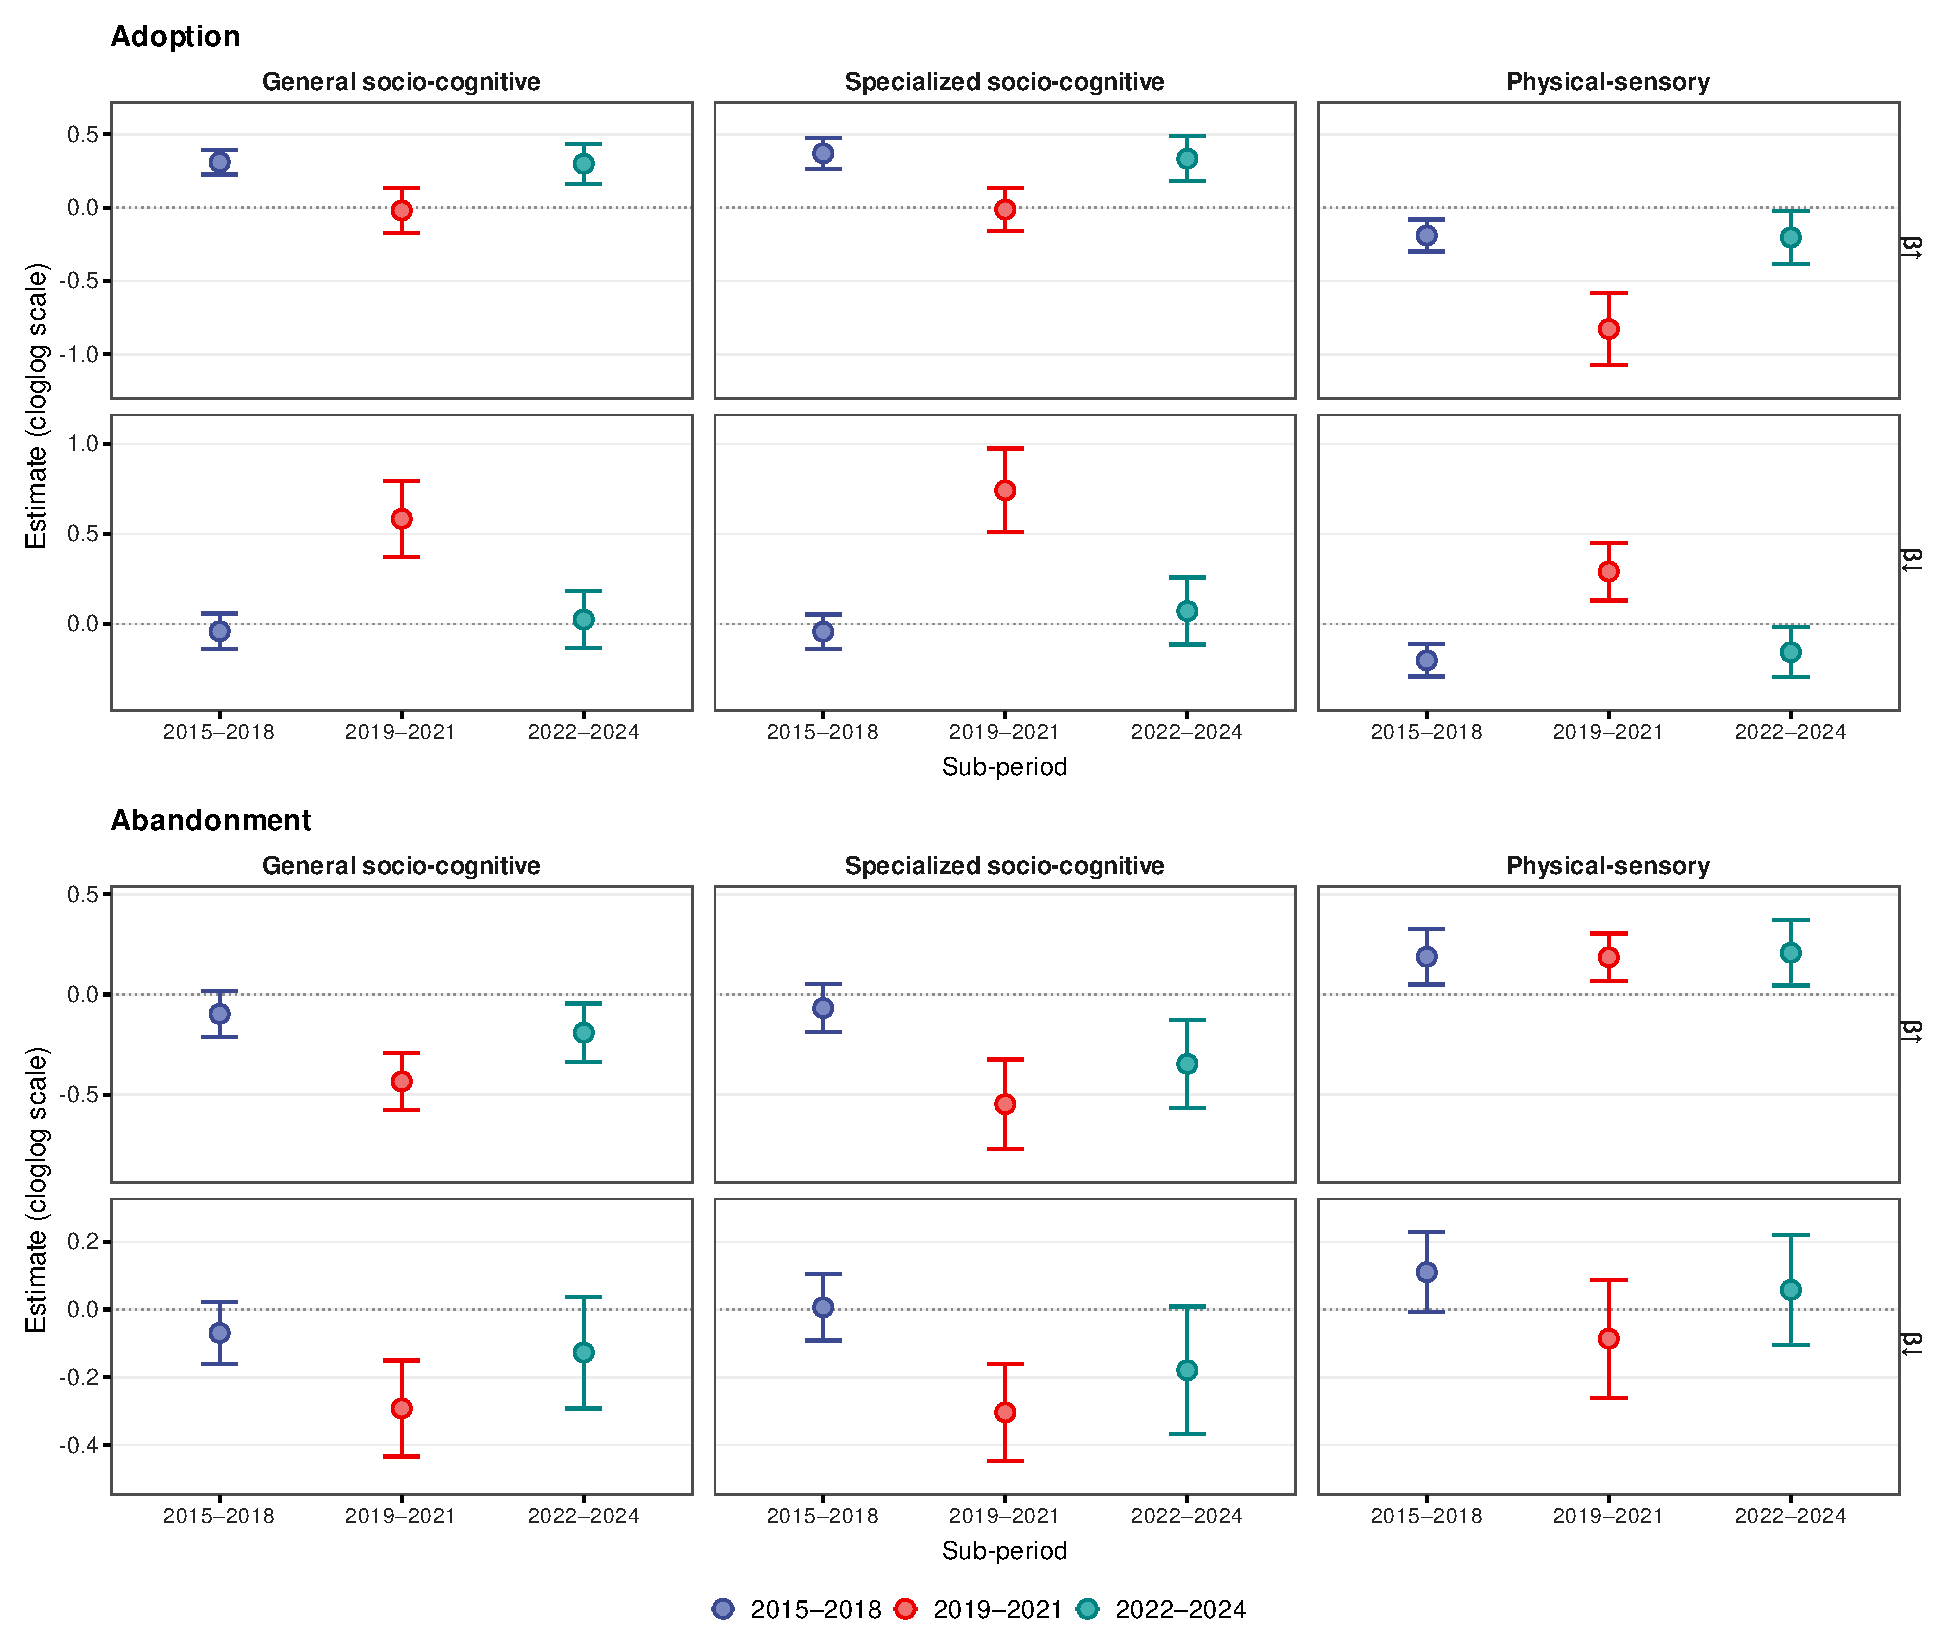
\includegraphics[width=0.95\textwidth]{figures/fig_SI_subperiods.pdf}
\caption{\textbf{Directional friction parameters are stable in direction across sub-periods.} Each panel shows Panel~A estimates ($\hat{\beta}^{\uparrow}$, top row; $\hat{\beta}^{\downarrow}$, bottom row) with 95\% confidence intervals (three-way clustering by source occupation, target occupation, and skill) for three non-overlapping sub-periods. Colors identify the sub-period. The sign of $\hat{\beta}^{\uparrow}$ is preserved across all periods and both flows: positive for socio-cognitive skills in adoption and negative in abandonment; reversed for sensory-physical skills. Wider intervals in 2019--2021 reflect reduced statistical power from the shorter observation window, not reversal of the gradient. The strengthening of $\hat{\beta}^{\uparrow}_{\text{Phys}}$ in adoption and of the socio-cognitive abandonment gradient in 2019--2021 is consistent with pandemic-period acceleration of directional diffusion, but the domain-reversing structure is present in all three windows. O*NET sub-period pairs: 2015--2018 (releases 20.3--23.1), 2019--2021 (24.1--26.1), 2022--2024 (27.1--29.2). \textbf{(A)}~Adoption. \textbf{(B)}~Abandonment.}
\label{fig:SI_subperiods}
\end{figure*}
